%%%%%
%% Appendices are optional. 
%% If none are present, comment out "%%%%%
%% Appendices are optional. 
%% If none are present, comment out "%%%%%
%% Appendices are optional. 
%% If none are present, comment out "%%%%%
%% Appendices are optional. 
%% If none are present, comment out "\include{appendices}" in main.tex
%%%%%
\appendix
\renewcommand{\thesubsection}{\Alph{subsection}}

\chapter{What Should Be Included in Appendices}\label{apx:appendix1}

Appendices should contain information that is too lengthy to be included in the thesis chapters but further support the conclusions of the thesis. For example, one could include additional experimental results in the form of tables or additional figures. Each appendix should start with a paragraph introducing the items being presented. Additionally, each table or figure should be preceded by a paragraph that explains the data being presented and the conclusions that can be drawn from them. Please note that data already presented in the main thesis should not be repeated in an appendix. One cannot, for example, include the results of an experiment as a figure in the thesis and again as a table in the appendix. One can, however, include detailed results in tables in the appendix and a summary figure in the thesis portraying only the ``best" results.

\section{Subsections in Appendices}\label{apx:appendix1:subsections}

It is possible, and advisable, to use (multiple levels of) subsections in an Appendix. The main Appendix sections may be optionally titled. They will automatically be assigned Appendix A, Appendix B, etc. If a title is present, it will appear on the next line in the appendix and on the same line in the TOC. Sub-sections will be listed in the TOC as A.1, A.2, etc.

Figures, such as \figurename~\ref{fig:nonzero-distr}, should only be referenced in the appendix. The thesis content can point to an appendix but not specifically reference a table or figure in the appendix.

\begin{figure}[!htb]
  \centering
  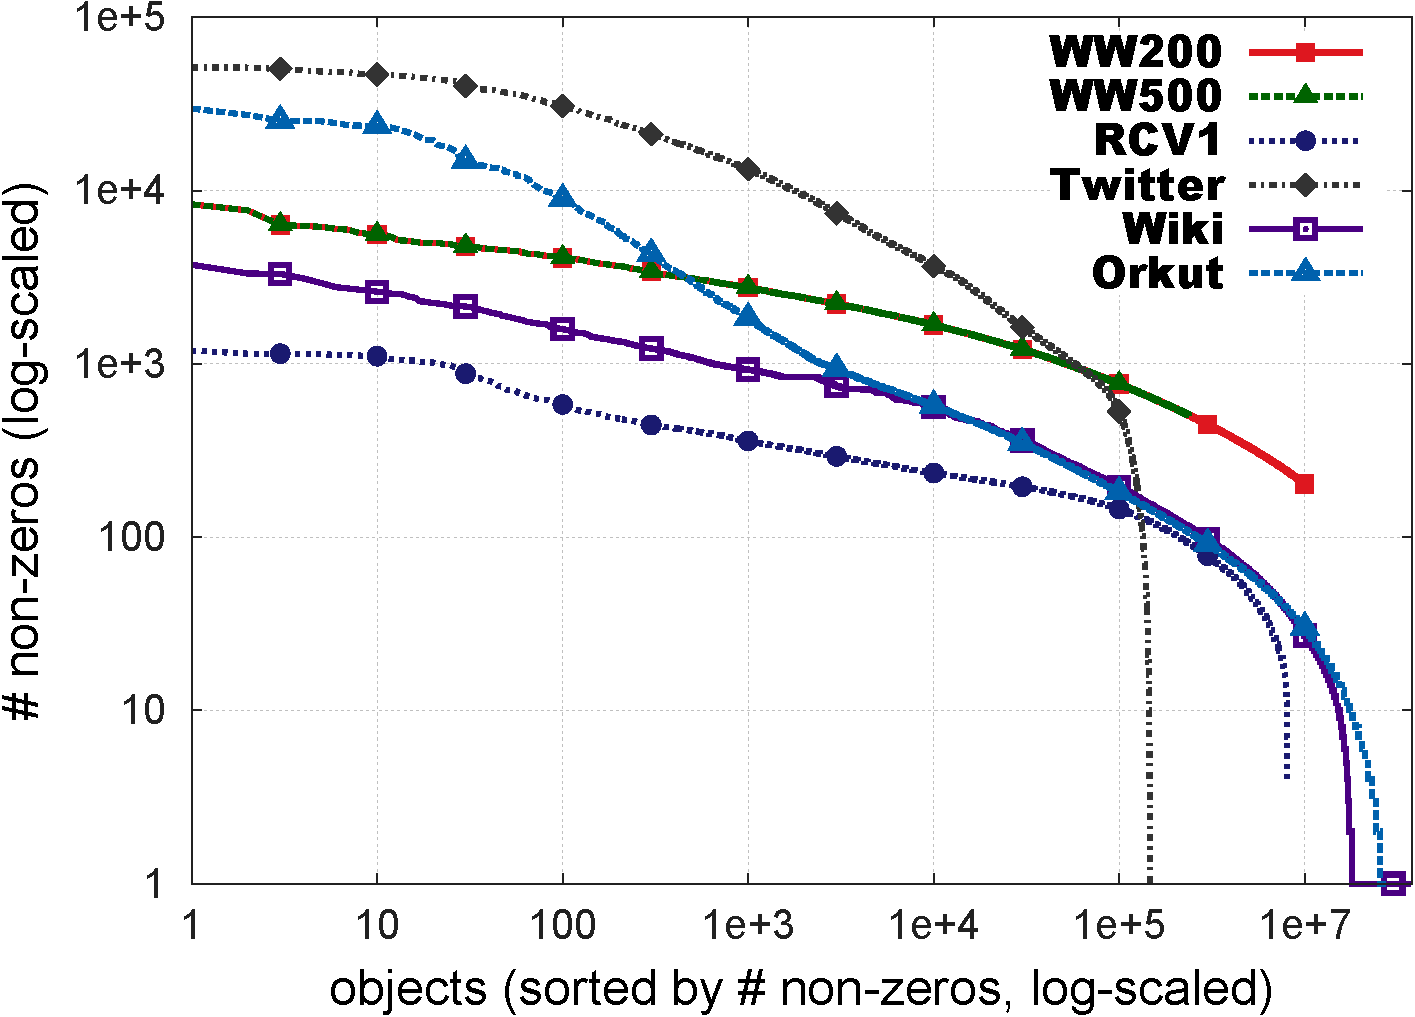
\includegraphics[width=0.6\textwidth]{img/hist-rows.pdf}
  \caption{Distribution of sample non-zeros.}
  \label{fig:nonzero-distr}
\end{figure}


\chapter{Title of Another Appendix}\label{apx:appendix2}

Different appendices should cover unrelated topics. If the appendices are on the same topic, they should just be sub-sections within the same appendix. 

\begin{figure}[tbh]
  \centering
  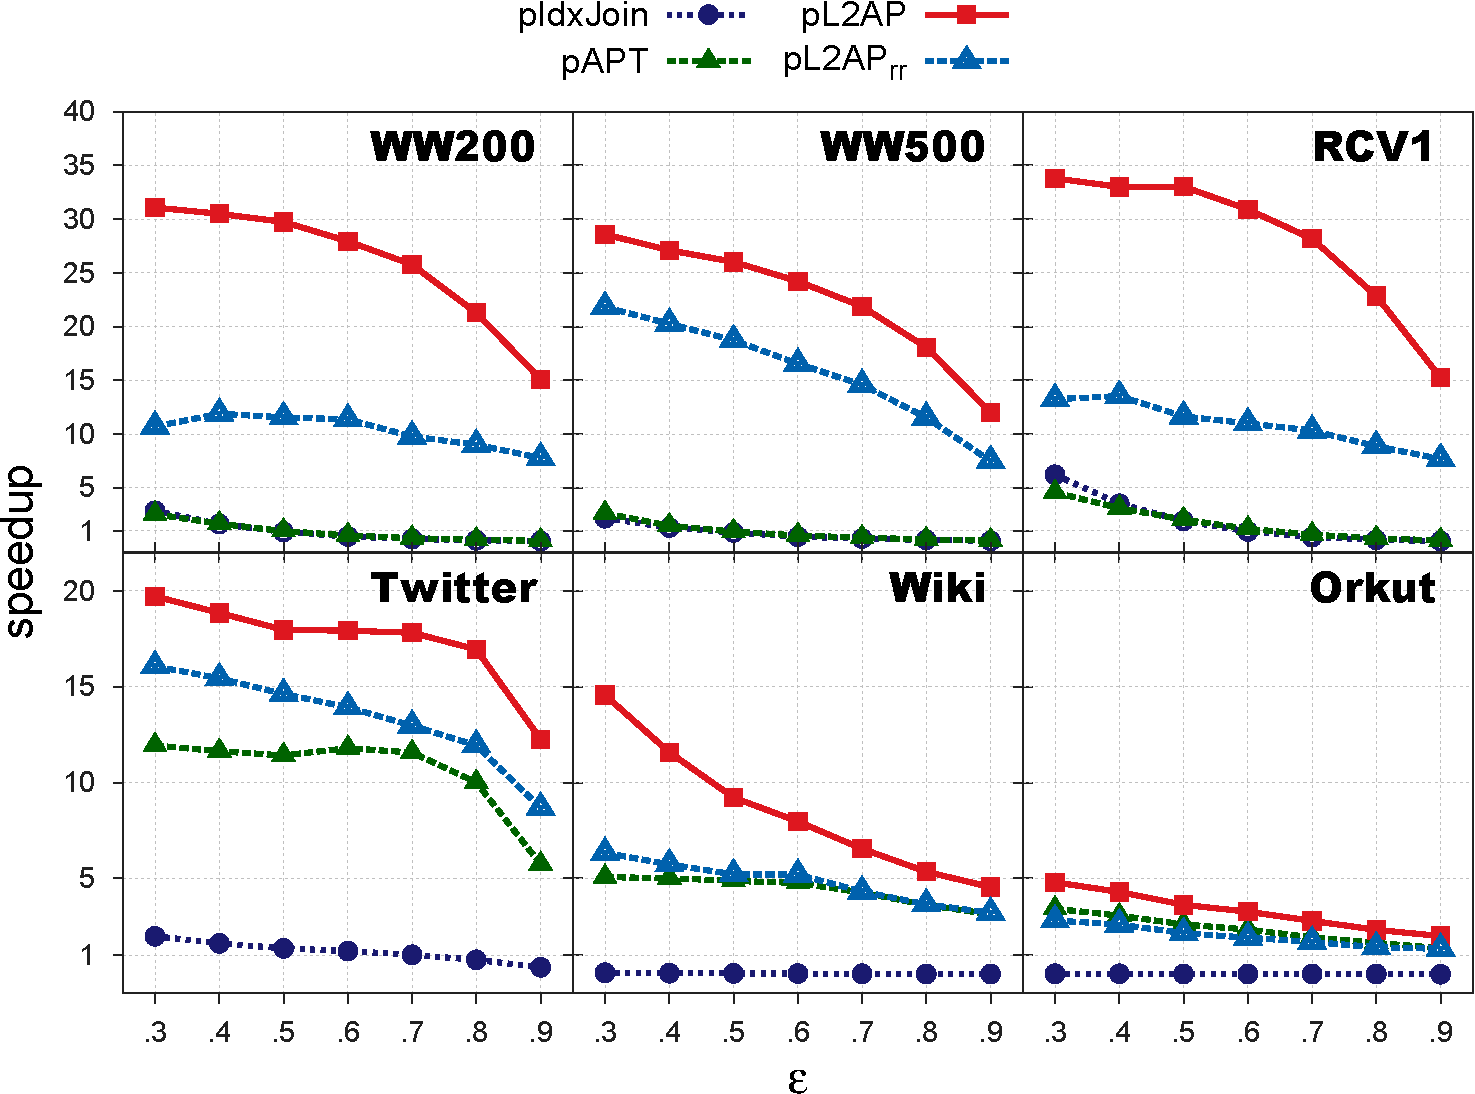
\includegraphics[width=0.85\textwidth]{img/speedup2-nbase.pdf}
  \caption{Speedup comparison of our method against baselines.}
  \label{fig:speedup}
\end{figure}" in main.tex
%%%%%
\appendix
\renewcommand{\thesubsection}{\Alph{subsection}}

\chapter{What Should Be Included in Appendices}\label{apx:appendix1}

Appendices should contain information that is too lengthy to be included in the thesis chapters but further support the conclusions of the thesis. For example, one could include additional experimental results in the form of tables or additional figures. Each appendix should start with a paragraph introducing the items being presented. Additionally, each table or figure should be preceded by a paragraph that explains the data being presented and the conclusions that can be drawn from them. Please note that data already presented in the main thesis should not be repeated in an appendix. One cannot, for example, include the results of an experiment as a figure in the thesis and again as a table in the appendix. One can, however, include detailed results in tables in the appendix and a summary figure in the thesis portraying only the ``best" results.

\section{Subsections in Appendices}\label{apx:appendix1:subsections}

It is possible, and advisable, to use (multiple levels of) subsections in an Appendix. The main Appendix sections may be optionally titled. They will automatically be assigned Appendix A, Appendix B, etc. If a title is present, it will appear on the next line in the appendix and on the same line in the TOC. Sub-sections will be listed in the TOC as A.1, A.2, etc.

Figures, such as \figurename~\ref{fig:nonzero-distr}, should only be referenced in the appendix. The thesis content can point to an appendix but not specifically reference a table or figure in the appendix.

\begin{figure}[!htb]
  \centering
  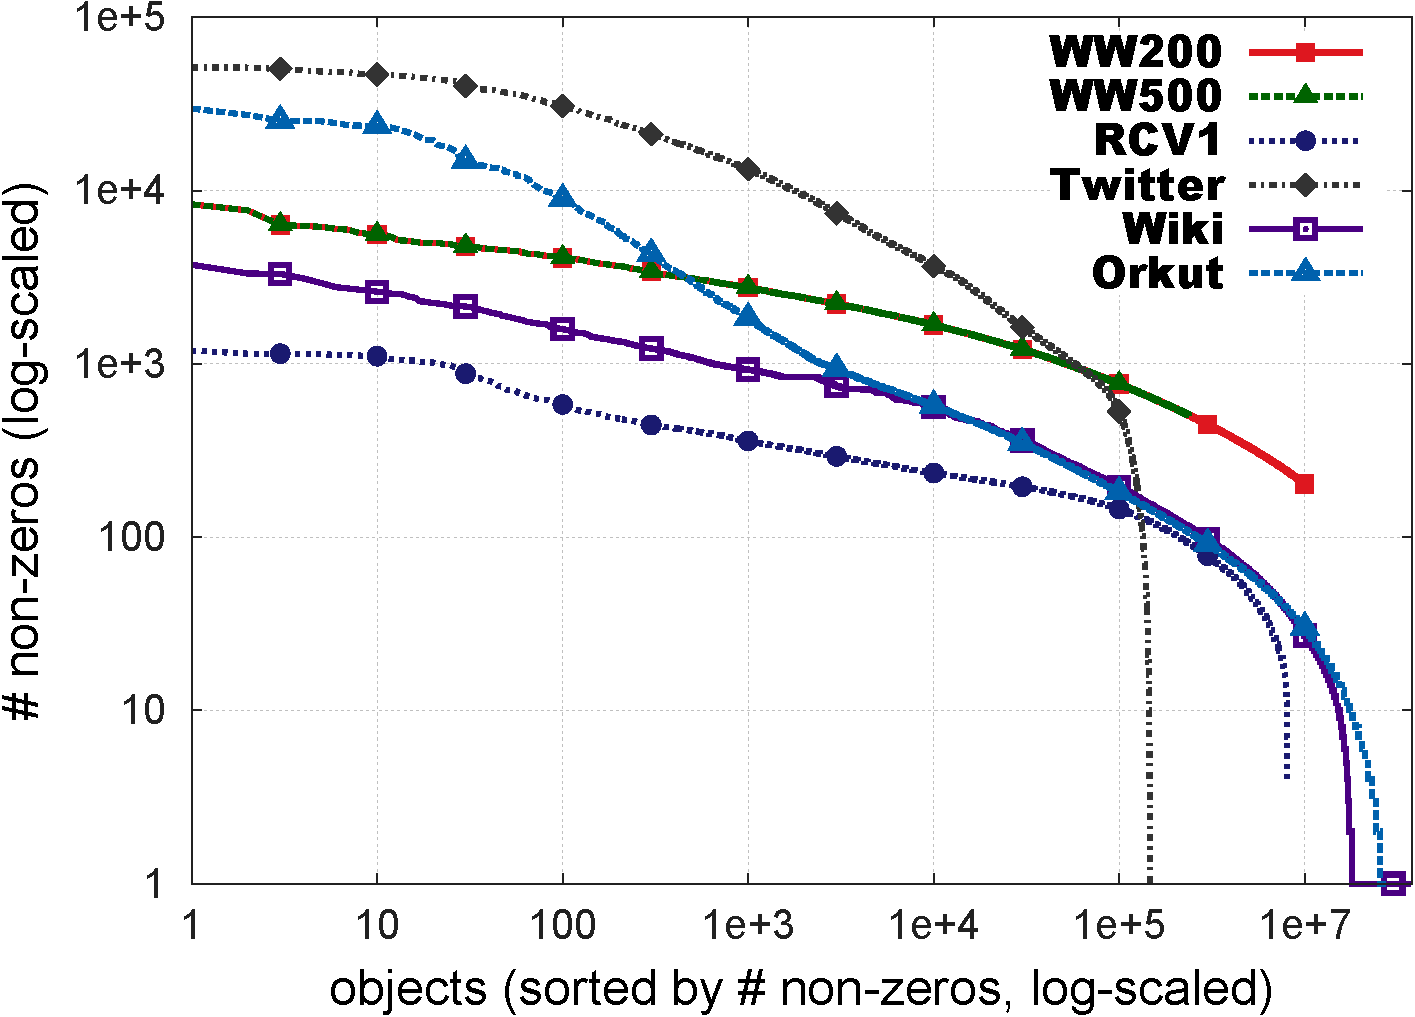
\includegraphics[width=0.6\textwidth]{img/hist-rows.pdf}
  \caption{Distribution of sample non-zeros.}
  \label{fig:nonzero-distr}
\end{figure}


\chapter{Title of Another Appendix}\label{apx:appendix2}

Different appendices should cover unrelated topics. If the appendices are on the same topic, they should just be sub-sections within the same appendix. 

\begin{figure}[tbh]
  \centering
  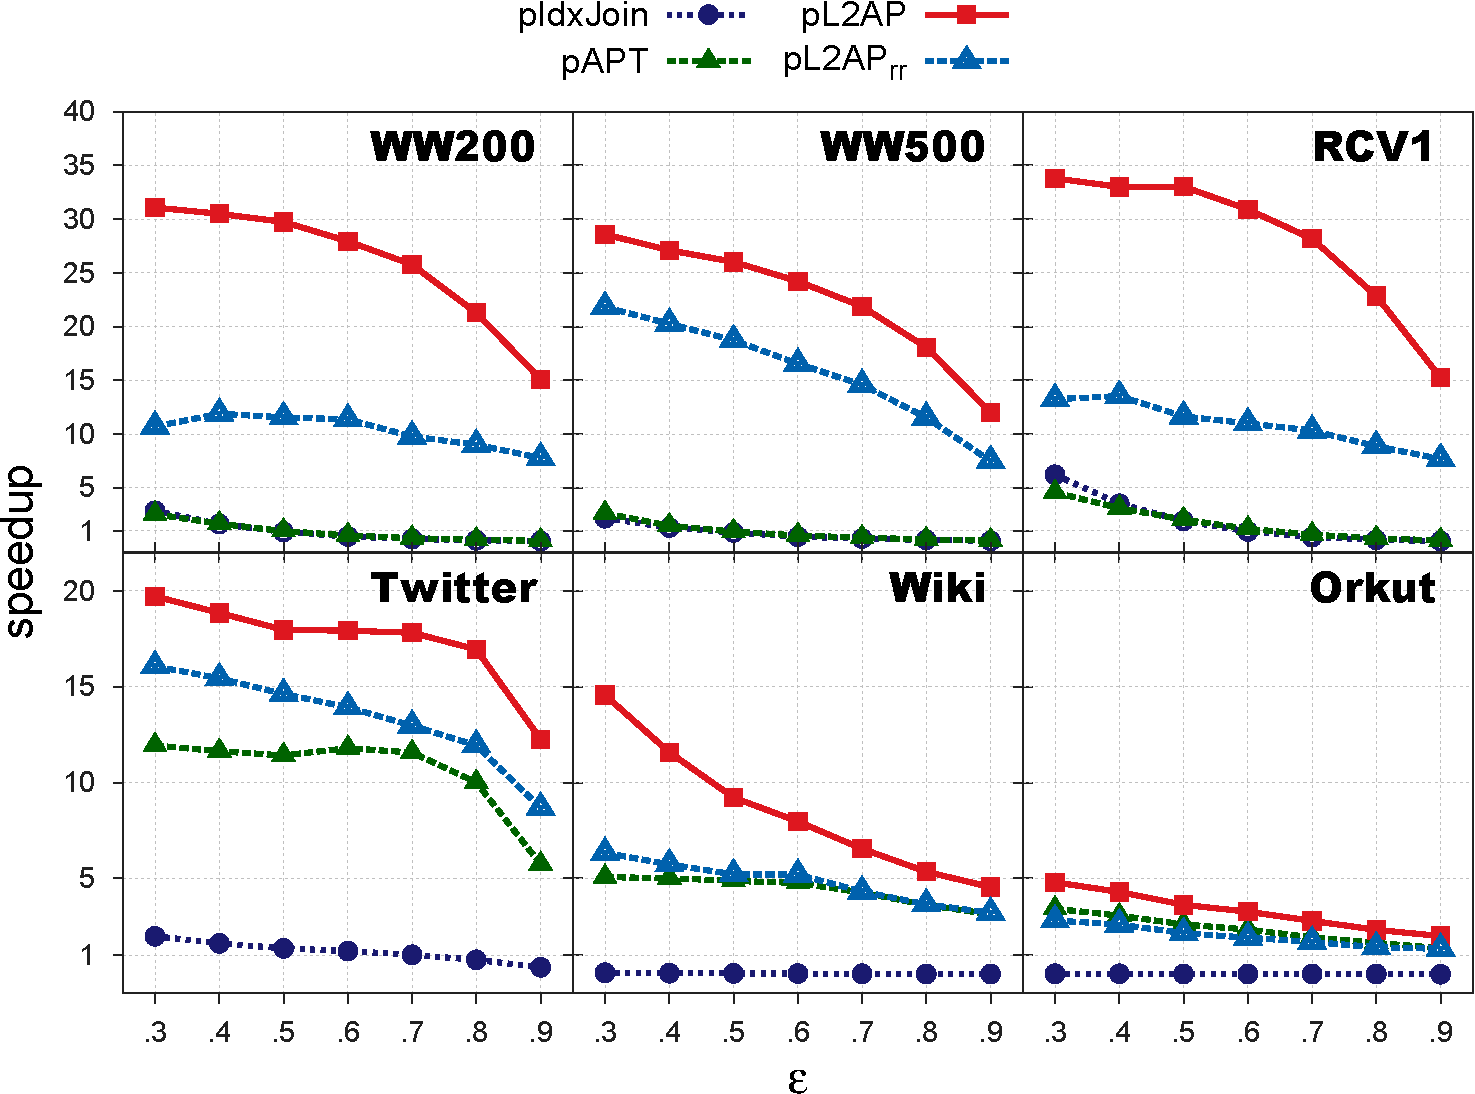
\includegraphics[width=0.85\textwidth]{img/speedup2-nbase.pdf}
  \caption{Speedup comparison of our method against baselines.}
  \label{fig:speedup}
\end{figure}" in main.tex
%%%%%
\appendix
\renewcommand{\thesubsection}{\Alph{subsection}}

\chapter{What Should Be Included in Appendices}\label{apx:appendix1}

Appendices should contain information that is too lengthy to be included in the thesis chapters but further support the conclusions of the thesis. For example, one could include additional experimental results in the form of tables or additional figures. Each appendix should start with a paragraph introducing the items being presented. Additionally, each table or figure should be preceded by a paragraph that explains the data being presented and the conclusions that can be drawn from them. Please note that data already presented in the main thesis should not be repeated in an appendix. One cannot, for example, include the results of an experiment as a figure in the thesis and again as a table in the appendix. One can, however, include detailed results in tables in the appendix and a summary figure in the thesis portraying only the ``best" results.

\section{Subsections in Appendices}\label{apx:appendix1:subsections}

It is possible, and advisable, to use (multiple levels of) subsections in an Appendix. The main Appendix sections may be optionally titled. They will automatically be assigned Appendix A, Appendix B, etc. If a title is present, it will appear on the next line in the appendix and on the same line in the TOC. Sub-sections will be listed in the TOC as A.1, A.2, etc.

Figures, such as \figurename~\ref{fig:nonzero-distr}, should only be referenced in the appendix. The thesis content can point to an appendix but not specifically reference a table or figure in the appendix.

\begin{figure}[!htb]
  \centering
  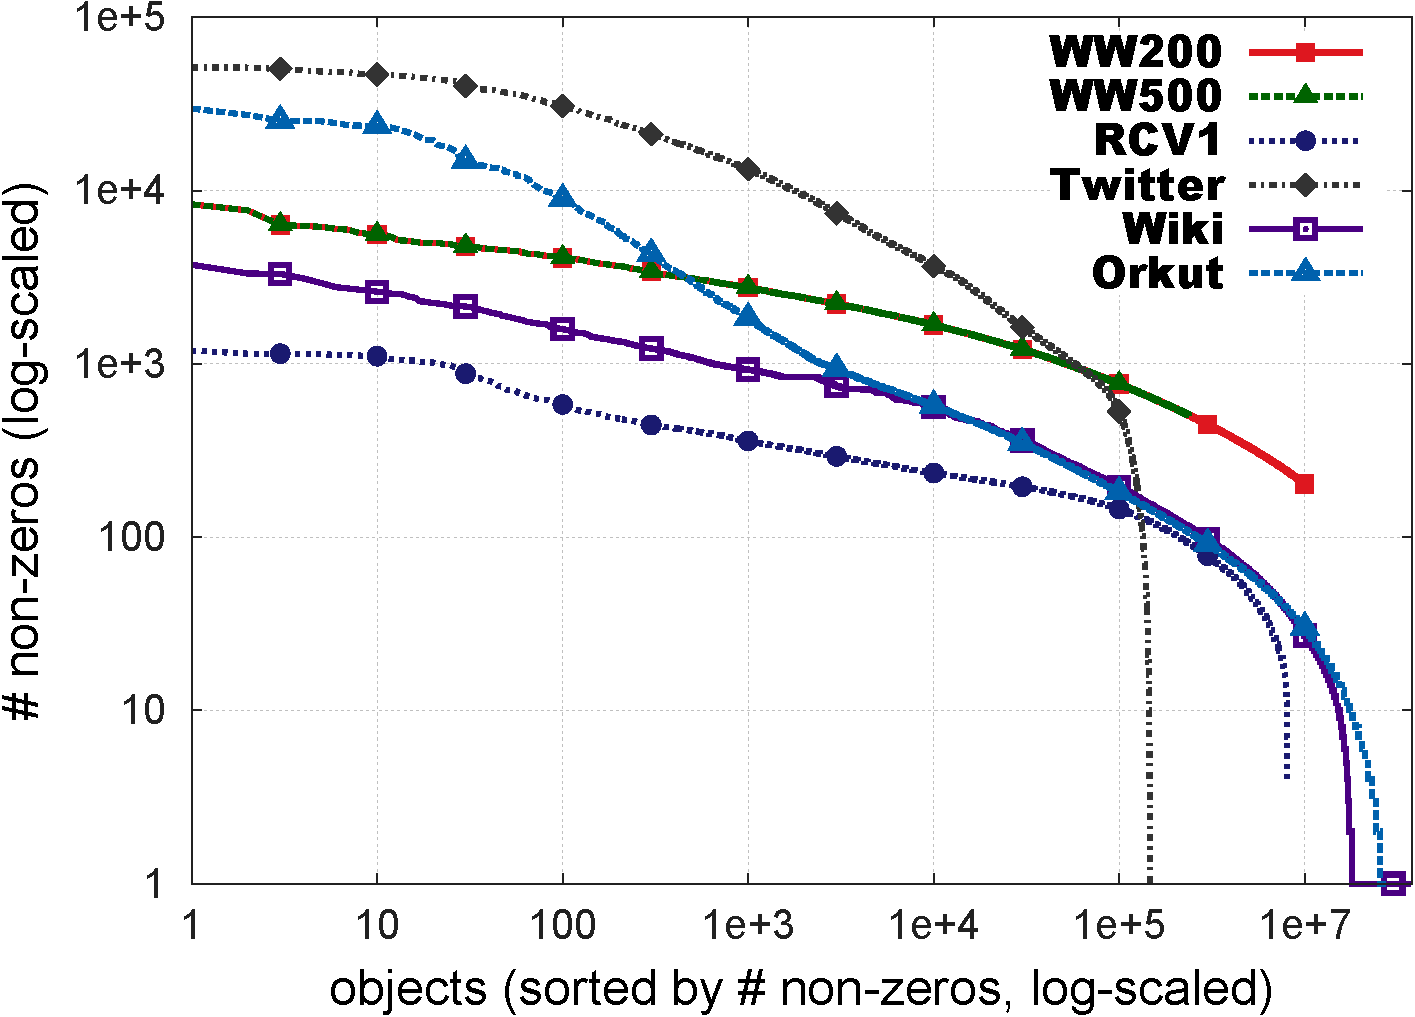
\includegraphics[width=0.6\textwidth]{img/hist-rows.pdf}
  \caption{Distribution of sample non-zeros.}
  \label{fig:nonzero-distr}
\end{figure}


\chapter{Title of Another Appendix}\label{apx:appendix2}

Different appendices should cover unrelated topics. If the appendices are on the same topic, they should just be sub-sections within the same appendix. 

\begin{figure}[tbh]
  \centering
  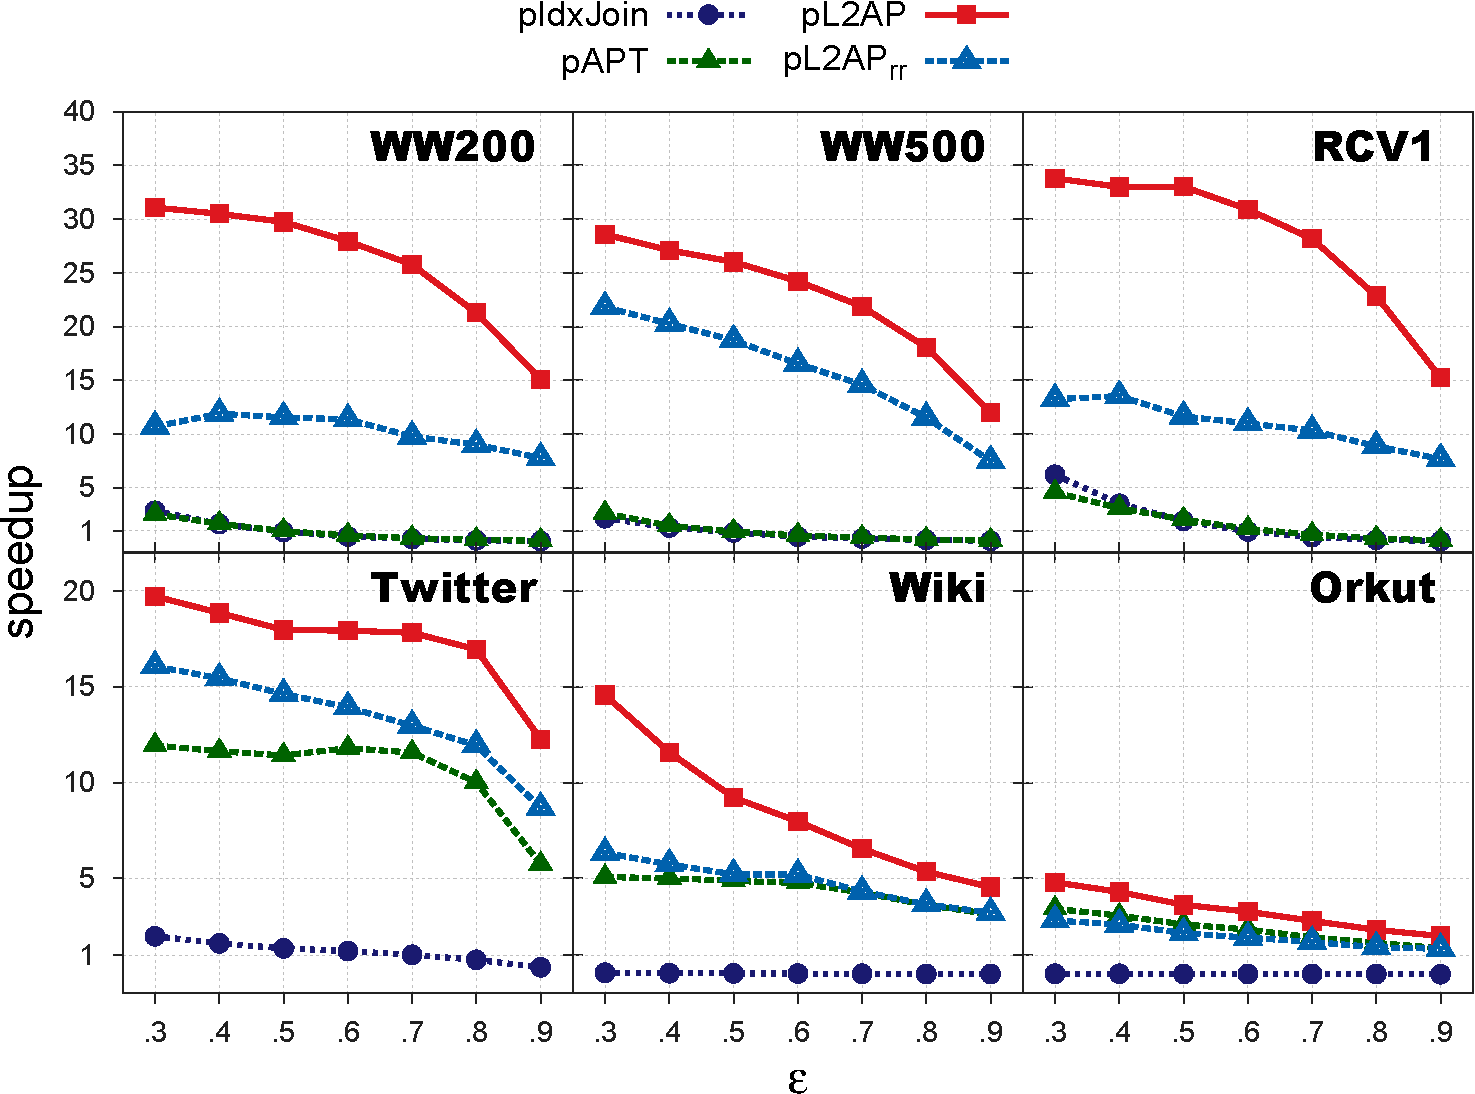
\includegraphics[width=0.85\textwidth]{img/speedup2-nbase.pdf}
  \caption{Speedup comparison of our method against baselines.}
  \label{fig:speedup}
\end{figure}" in main.tex
%%%%%
\appendix
\renewcommand{\thesubsection}{\Alph{subsection}}

\chapter{What Should Be Included in Appendices}\label{apx:appendix1}

Appendices should contain information that is too lengthy to be included in the thesis chapters but further support the conclusions of the thesis. For example, one could include additional experimental results in the form of tables or additional figures. Each appendix should start with a paragraph introducing the items being presented. Additionally, each table or figure should be preceded by a paragraph that explains the data being presented and the conclusions that can be drawn from them. Please note that data already presented in the main thesis should not be repeated in an appendix. One cannot, for example, include the results of an experiment as a figure in the thesis and again as a table in the appendix. One can, however, include detailed results in tables in the appendix and a summary figure in the thesis portraying only the ``best" results.

\section{Subsections in Appendices}\label{apx:appendix1:subsections}

It is possible, and advisable, to use (multiple levels of) subsections in an Appendix. The main Appendix sections may be optionally titled. They will automatically be assigned Appendix A, Appendix B, etc. If a title is present, it will appear on the next line in the appendix and on the same line in the TOC. Sub-sections will be listed in the TOC as A.1, A.2, etc.

Figures, such as \figurename~\ref{fig:nonzero-distr}, should only be referenced in the appendix. The thesis content can point to an appendix but not specifically reference a table or figure in the appendix.

\begin{figure}[!htb]
  \centering
  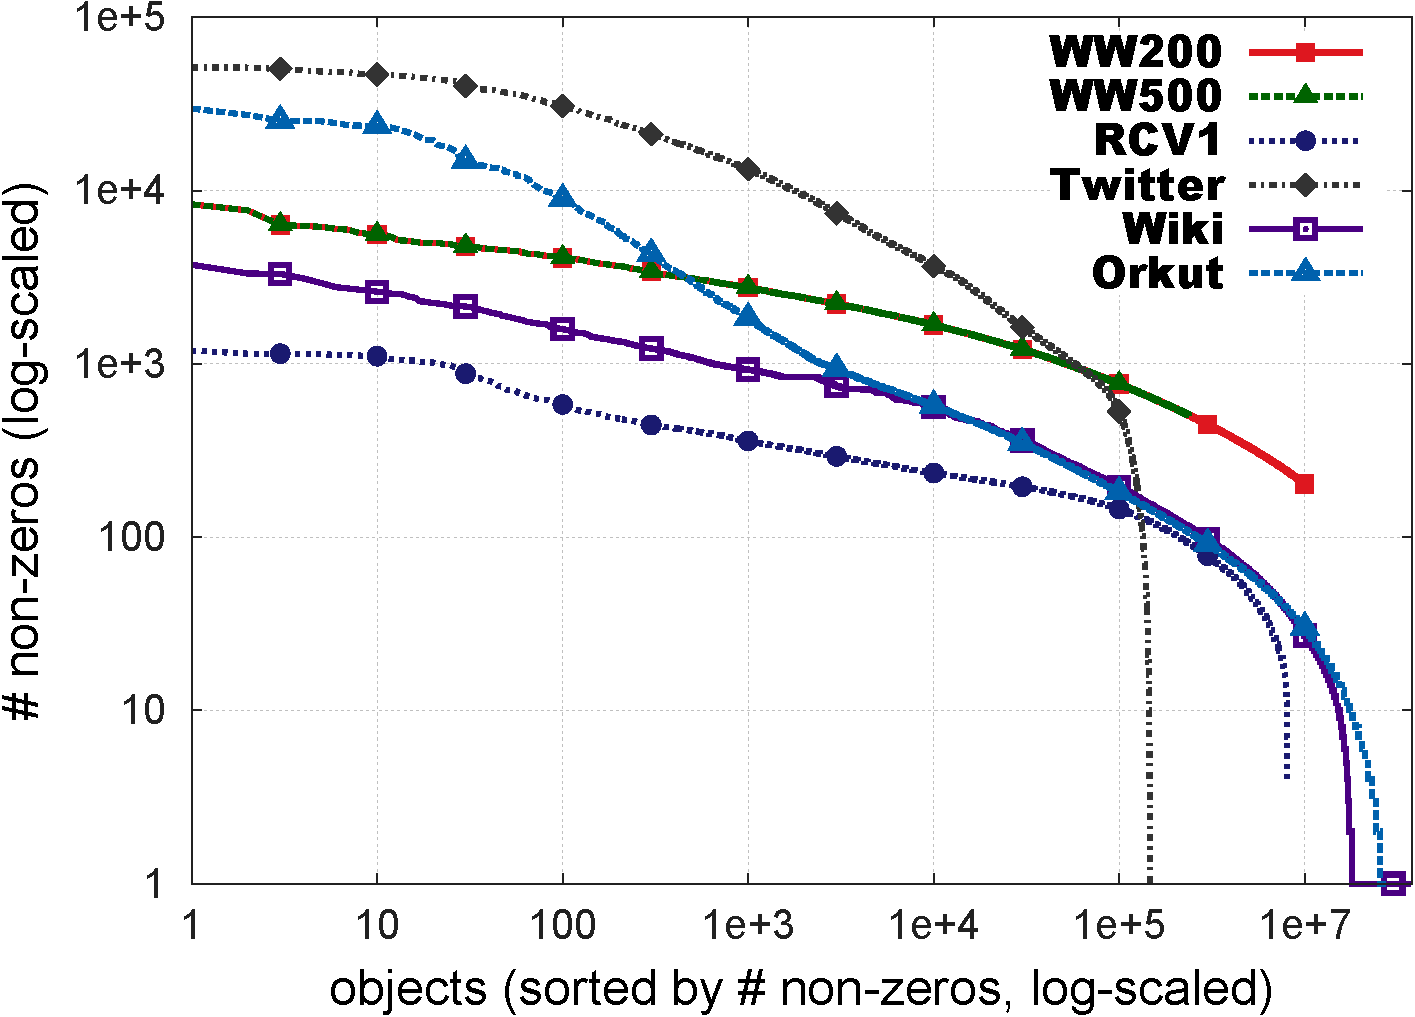
\includegraphics[width=0.6\textwidth]{img/hist-rows.pdf}
  \caption{Distribution of sample non-zeros.}
  \label{fig:nonzero-distr}
\end{figure}


\chapter{Title of Another Appendix}\label{apx:appendix2}

Different appendices should cover unrelated topics. If the appendices are on the same topic, they should just be sub-sections within the same appendix. 

\begin{figure}[tbh]
  \centering
  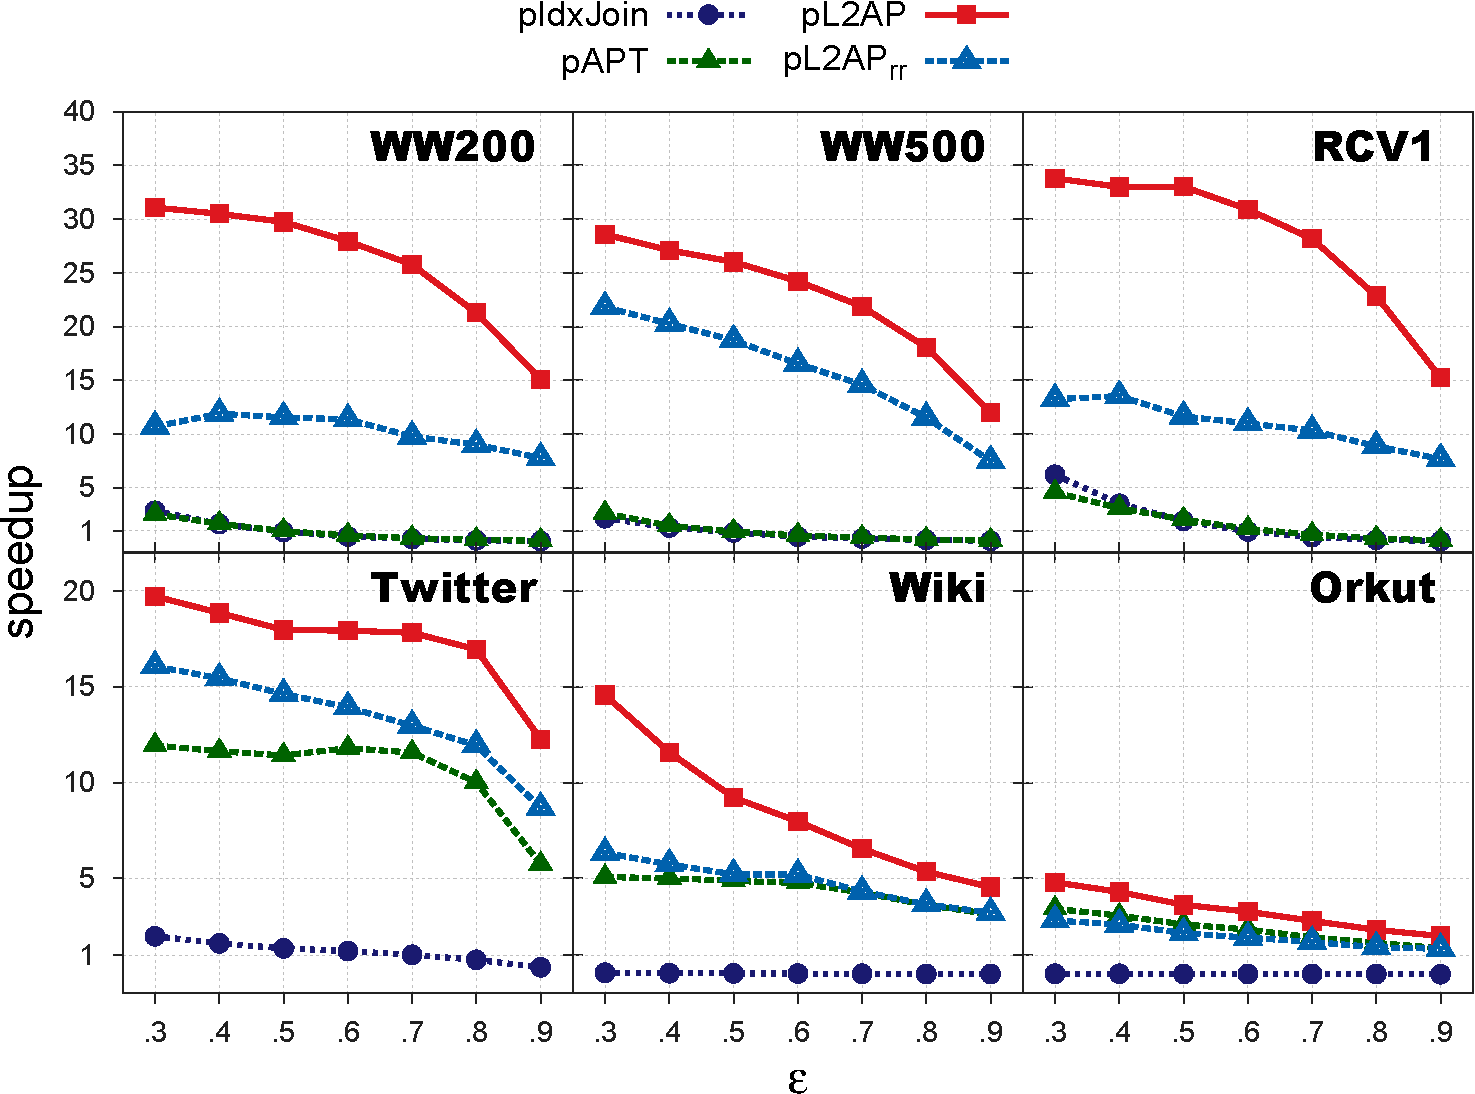
\includegraphics[width=0.85\textwidth]{img/speedup2-nbase.pdf}
  \caption{Speedup comparison of our method against baselines.}
  \label{fig:speedup}
\end{figure}